
\section{Results and Discussion}
\subsection{Anomaly Detection Performance}
After changing to using \texttt{isolation\_forest.anomaly\_score()} instead of \texttt{.predict()}, our scratch implementation of the Isolation Forest algorithm achieved a PR curve area of 0.43 and an ROC-AUC of 0.673. In comparison, the scikit-learn implementation yielded a PR curve area of 0.51 and an ROC-AUC of 0.72.

Figure \ref{fig:sklearn_pr} shows the PR curve for the scikit-learn implementation, while Figure \ref{fig:sklearn_roc} displays the corresponding ROC curve. Similarly, Figure \ref{fig:scratch_pr} presents the PR curve for our scratch implementation, and Figure \ref{fig:scratch_roc} shows the ROC curve.

\begin{figure}[htbp]
\centering
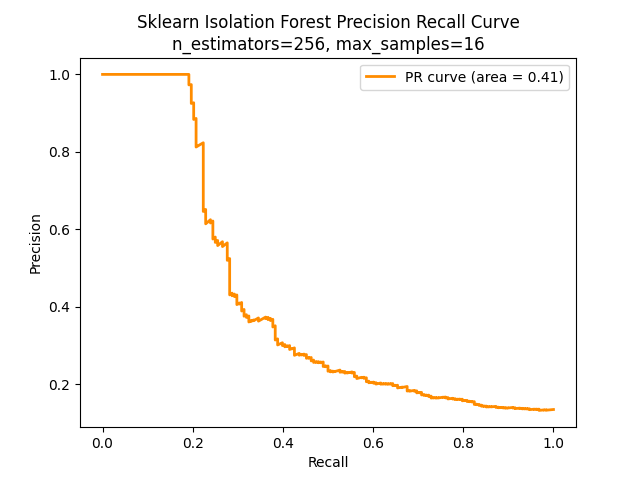
\includegraphics[width=0.5\textwidth]{resources/images/_sklearn_isolation_forest_pr_curve.png}
\caption{PR curve for the scikit-learn implementation}
\label{fig:sklearn_pr}
\end{figure}

\begin{figure}[htbp]
\centering
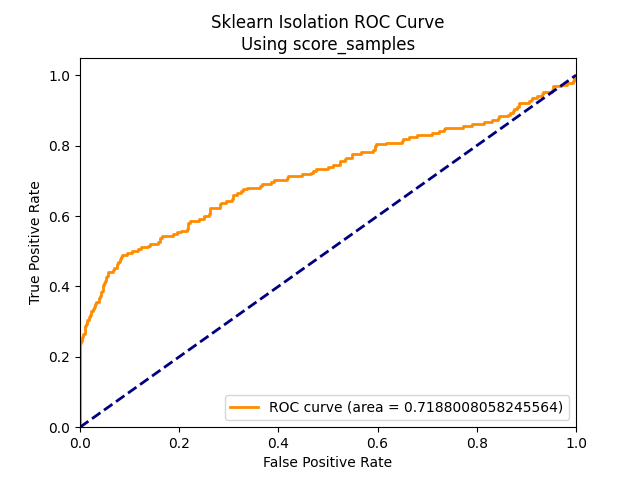
\includegraphics[width=0.5\textwidth]{resources/images/_sklearn_isolation_forest_roc_curve.png}
\caption{ROC curve for the scikit-learn implementation}
\label{fig:sklearn_roc}
\end{figure}

\begin{figure}[htbp]
\centering
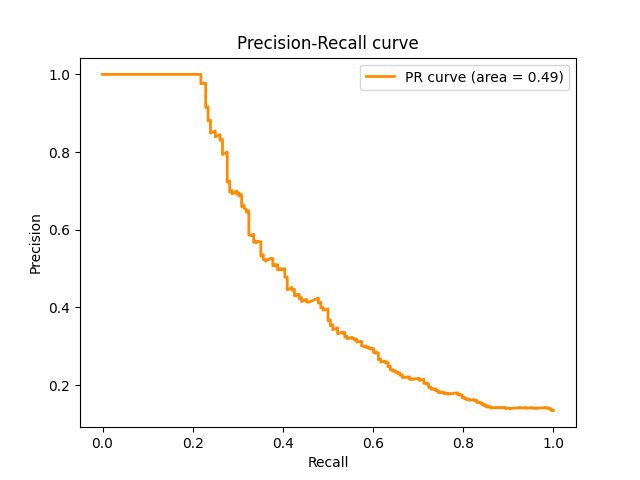
\includegraphics[width=0.5\textwidth]{resources/images/scratch_pr_curve.png}
\caption{PR curve for our scratch implementation}
\label{fig:scratch_pr}
\end{figure}

\begin{figure}[htbp]
\centering
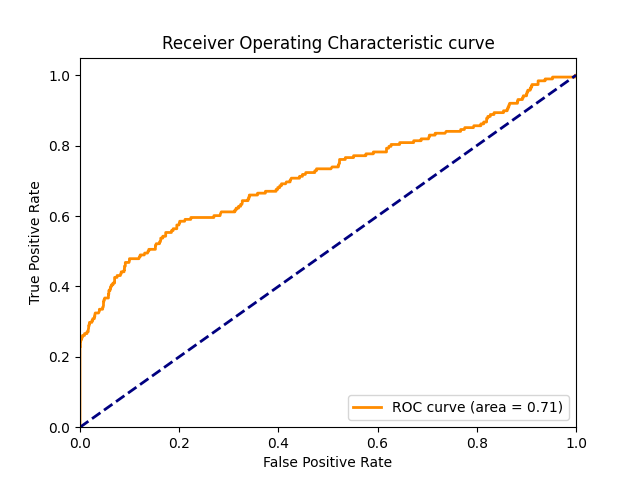
\includegraphics[width=0.5\textwidth]{resources/images/scratch_roc_curve.png}
\caption{ROC curve for our scratch implementation}
\label{fig:scratch_roc}
\end{figure}

\subsection{Visualization of Isolation Forest}
Figure \ref{fig:itree} depicts an example of an iTree, where each node represents a partition of the data based on a randomly selected feature and split point. The leaf nodes represent the isolated instances, with anomalies typically being isolated closer to the root of the tree.

\begin{figure}[htbp]
\centering
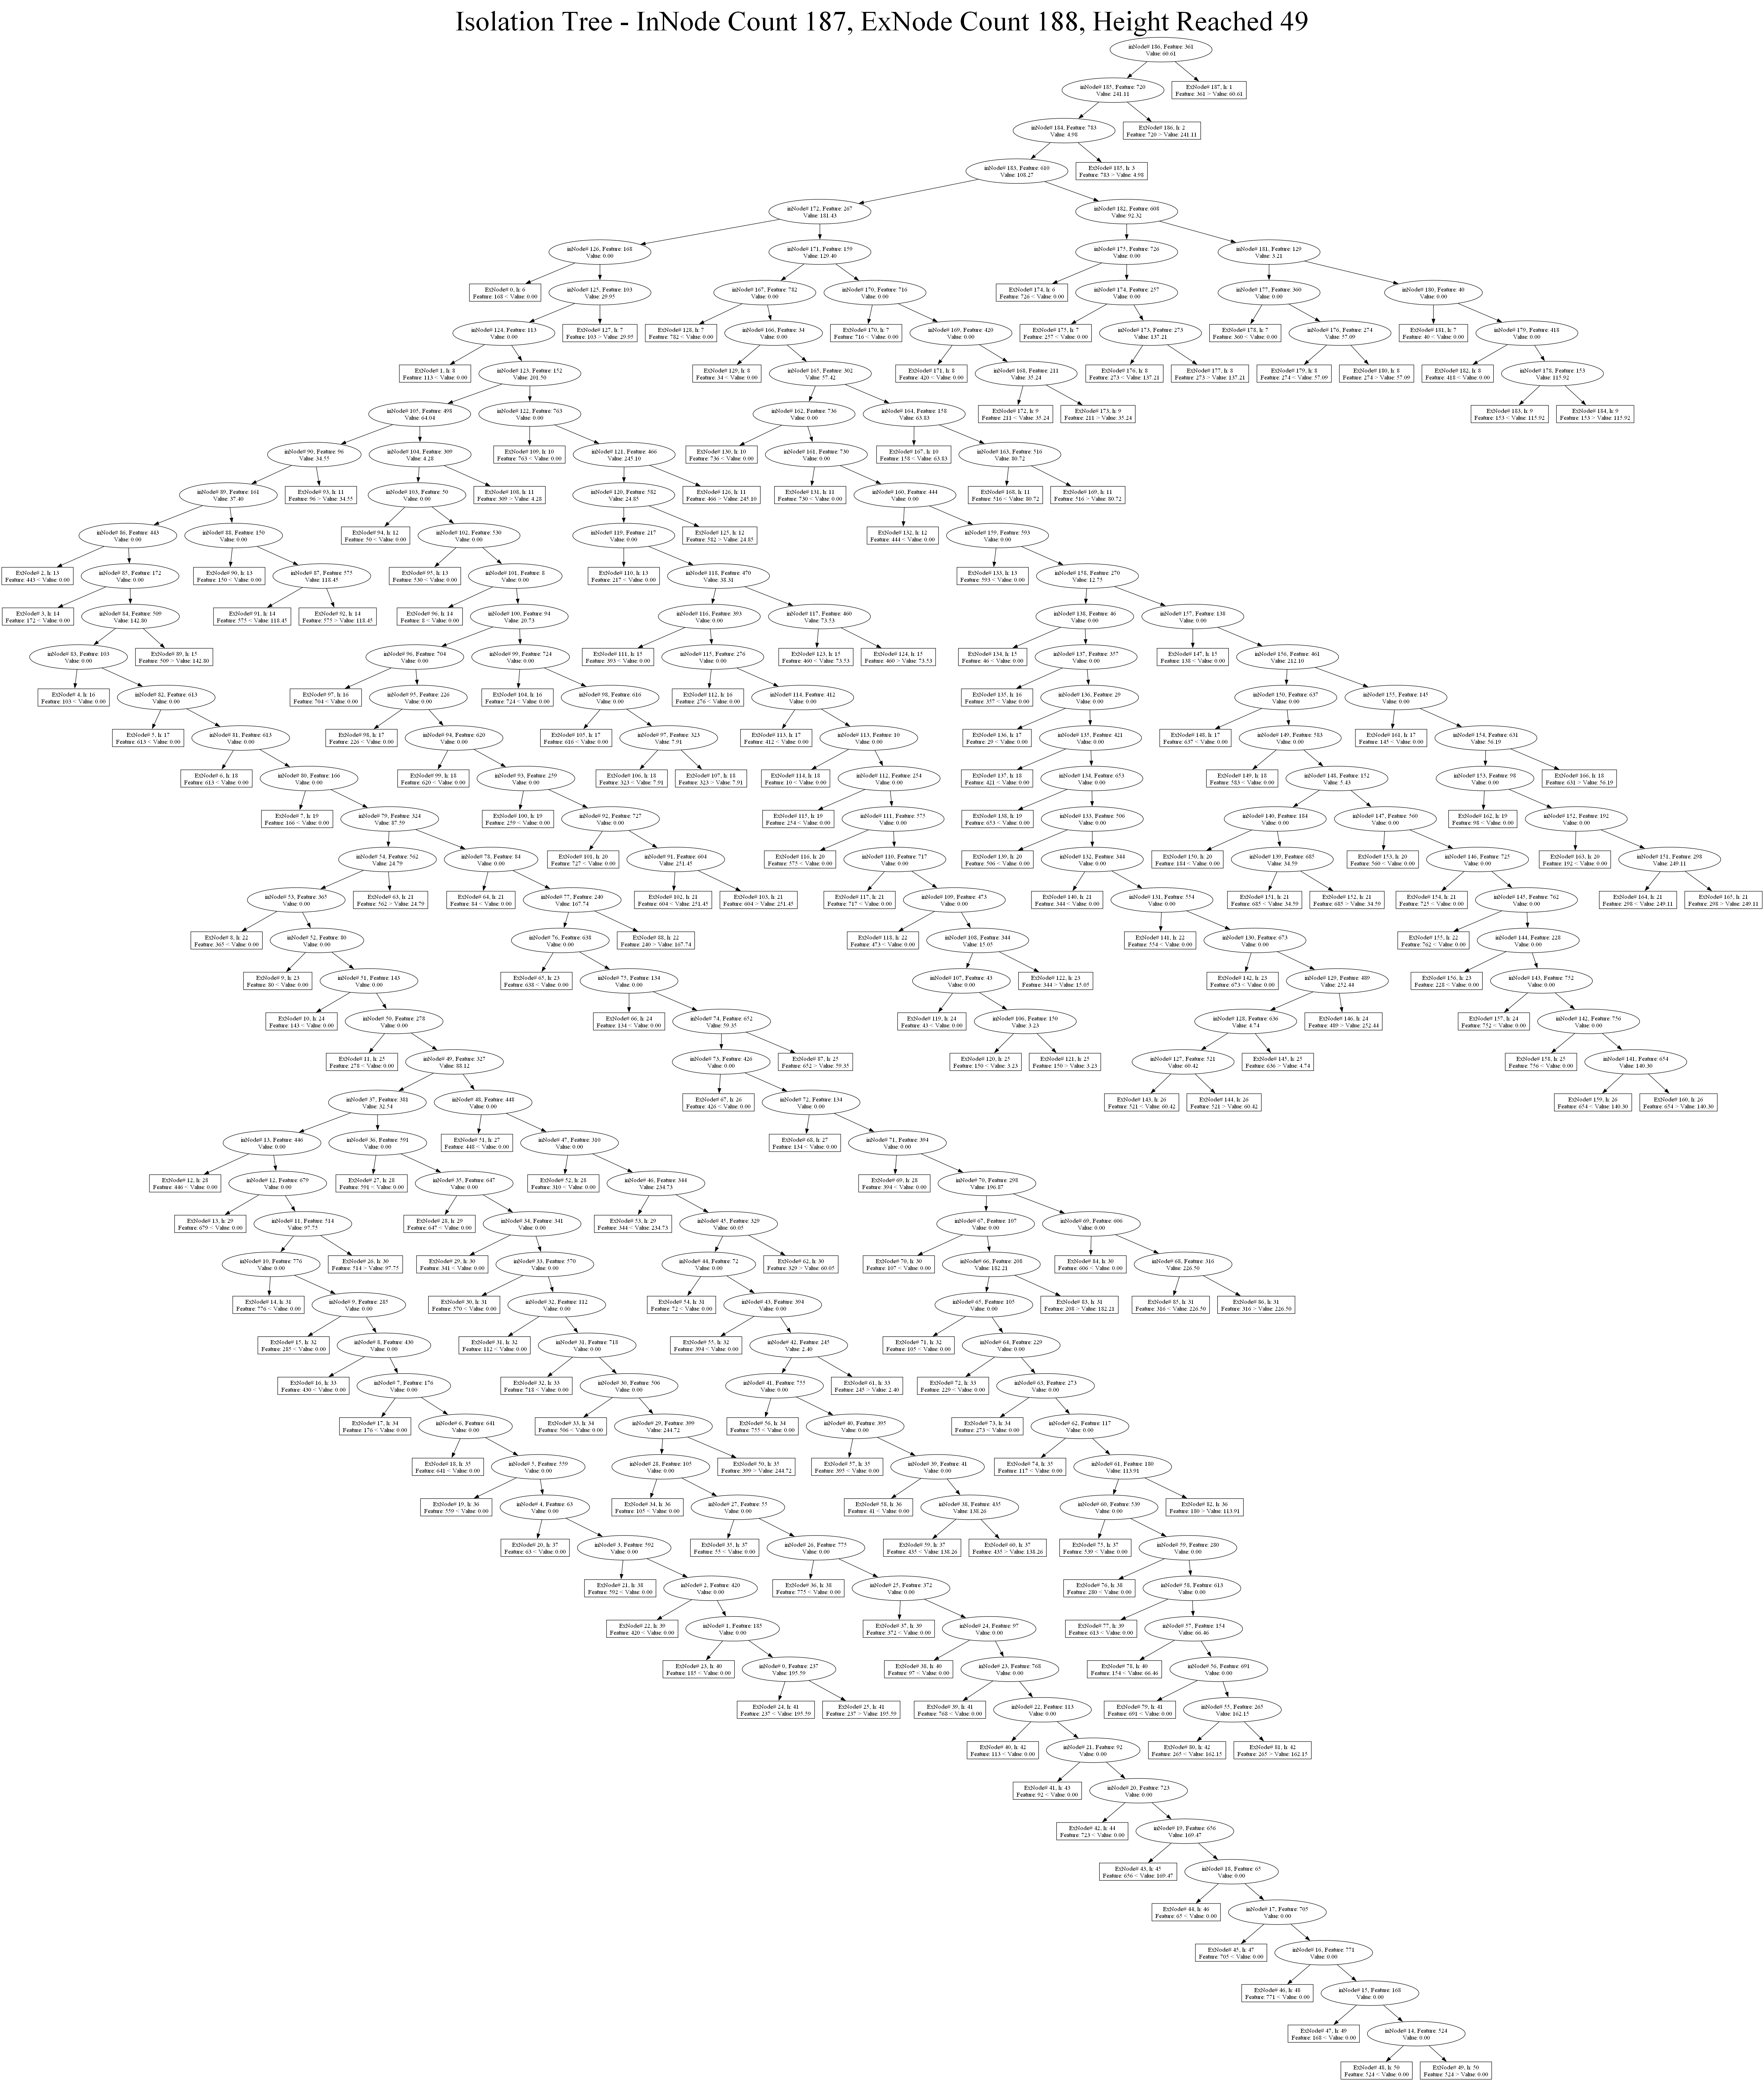
\includegraphics[width=0.5\textwidth]{resources/images/itree_graph.png}
\caption{Visualization of an Isolation Tree (iTree)}
\label{fig:itree}
\end{figure}

The visualization helps understand how the Isolation Forest algorithm partitions the data and isolates anomalies.

\subsection{Dimensionality Reduction}
To visualize the anomaly scores in a 2-dimensional space, we applied dimensionality reduction techniques such as t-SNE and PCA to the dataset prior to fitting the Isolation Forest algorithm.

With t-SNE using 2 components, the resulting tree heights were 6. The PR curve area was 0.33, and the ROC-AUC was 0.46. The performance was poor, and the contour plot (Figure \ref{fig:tsne_contour}) shows that the nominal and anomaly points are mixed together.

\begin{figure}[htbp]
\centering
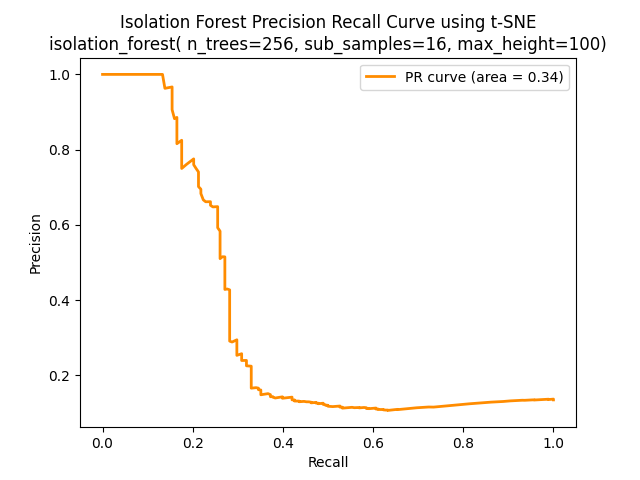
\includegraphics[width=0.5\textwidth]{resources/images/scratch_tsne_pr_curve.png}
\caption{PR curve for t-SNE with 2 components}
\label{fig:tsne_pr}
\end{figure}

\begin{figure}[htbp]
\centering
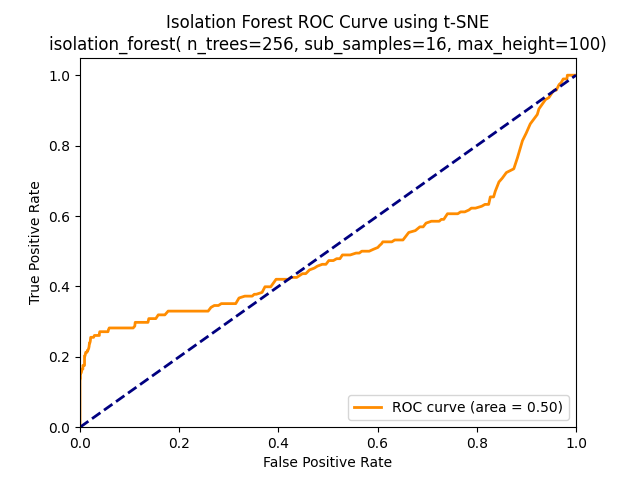
\includegraphics[width=0.5\textwidth]{resources/images/scratch_tsne_roc_curve.png}
\caption{ROC curve for t-SNE with 2 components}
\label{fig:tsne_roc}
\end{figure}

\begin{figure}[htbp]
\centering
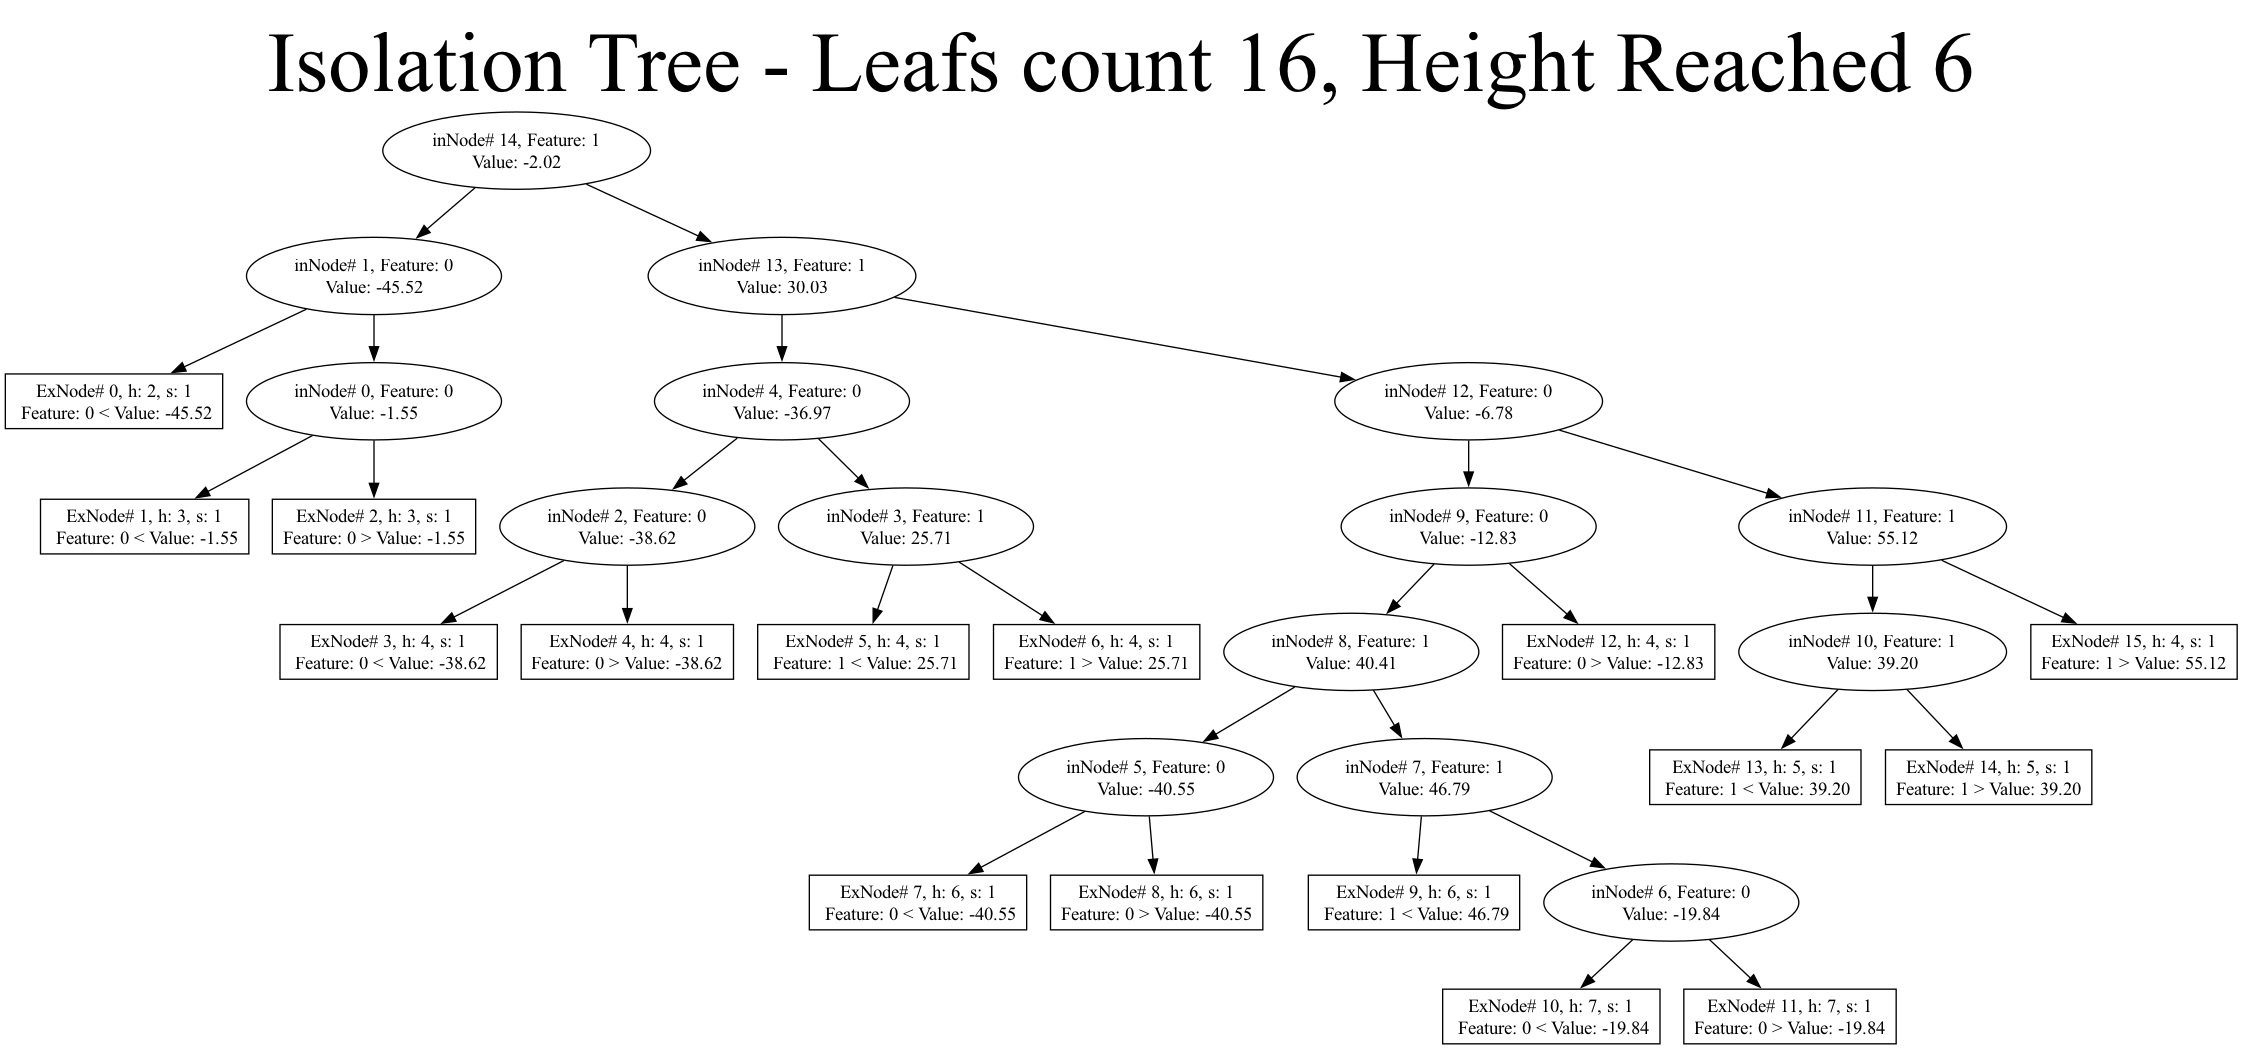
\includegraphics[width=0.5\textwidth]{resources/images/itree_tsne_graph.png}
\caption{Visualization of an iTree with t-SNE}
\label{fig:tsne_itree}
\end{figure}

\begin{figure}[htbp]
\centering
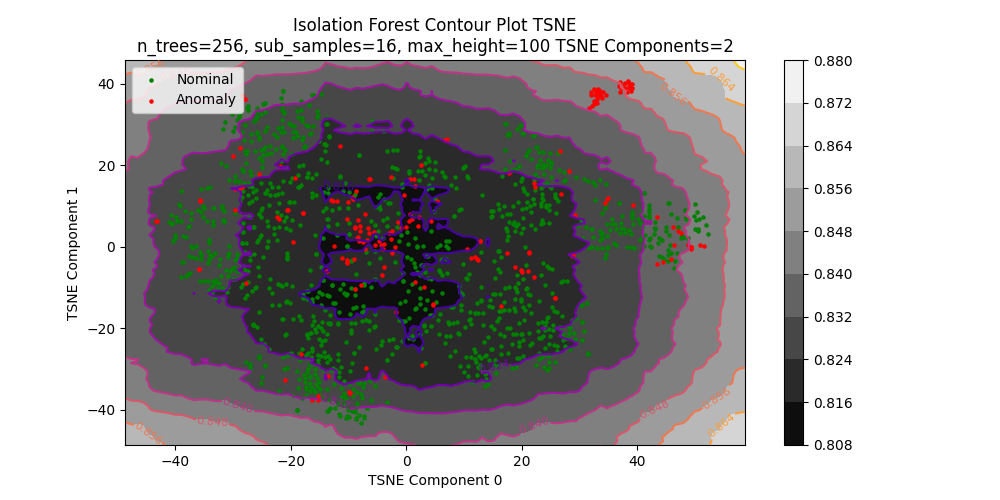
\includegraphics[width=0.5\textwidth]{resources/images/_TSNE_contour_plot.png}
\caption{Contour plot of anomaly scores with t-SNE}
\label{fig:tsne_contour}
\end{figure}

With PCA using 2 components, the resulting tree heights were approximately 10. The PR-AUC was 0.34, and the ROC-AUC was 0.62. The contour plot (Figure \ref{fig:pca_contour}) shows mixing of nominal and anomaly points, but there is some distinction.

\begin{figure}[htbp]
\centering
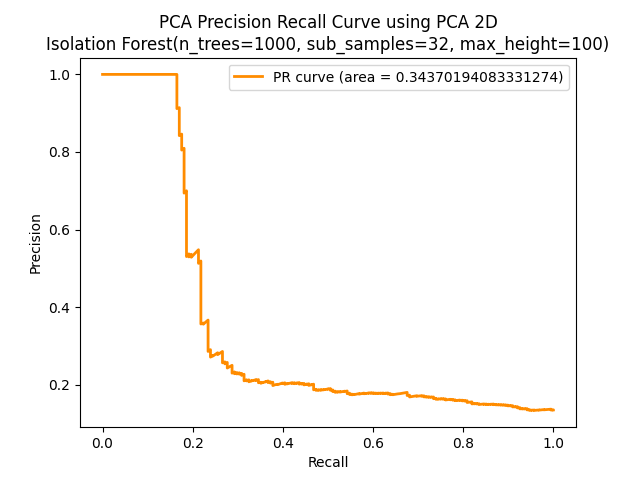
\includegraphics[width=0.5\textwidth]{resources/images/pca_pr_curve.png}
\caption{PR curve for PCA with 2 components}
\label{fig:pca_pr}
\end{figure}

\begin{figure}[htbp]
\centering
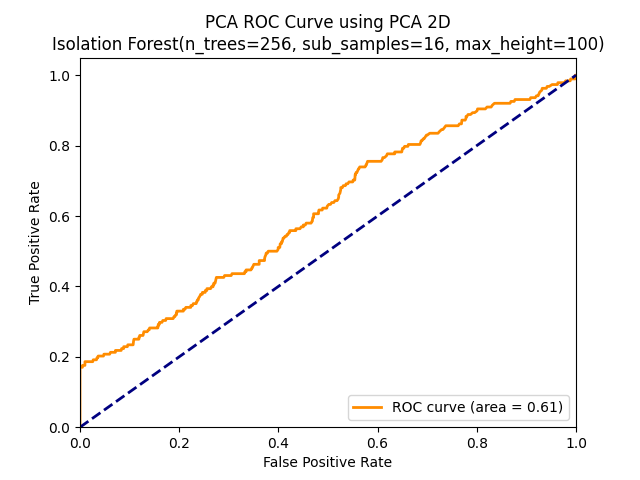
\includegraphics[width=0.5\textwidth]{resources/images/pca_roc_curve.png}
\caption{ROC curve for PCA with 2 components}
\label{fig:pca_roc}
\end{figure}

\begin{figure}[htbp]
\centering
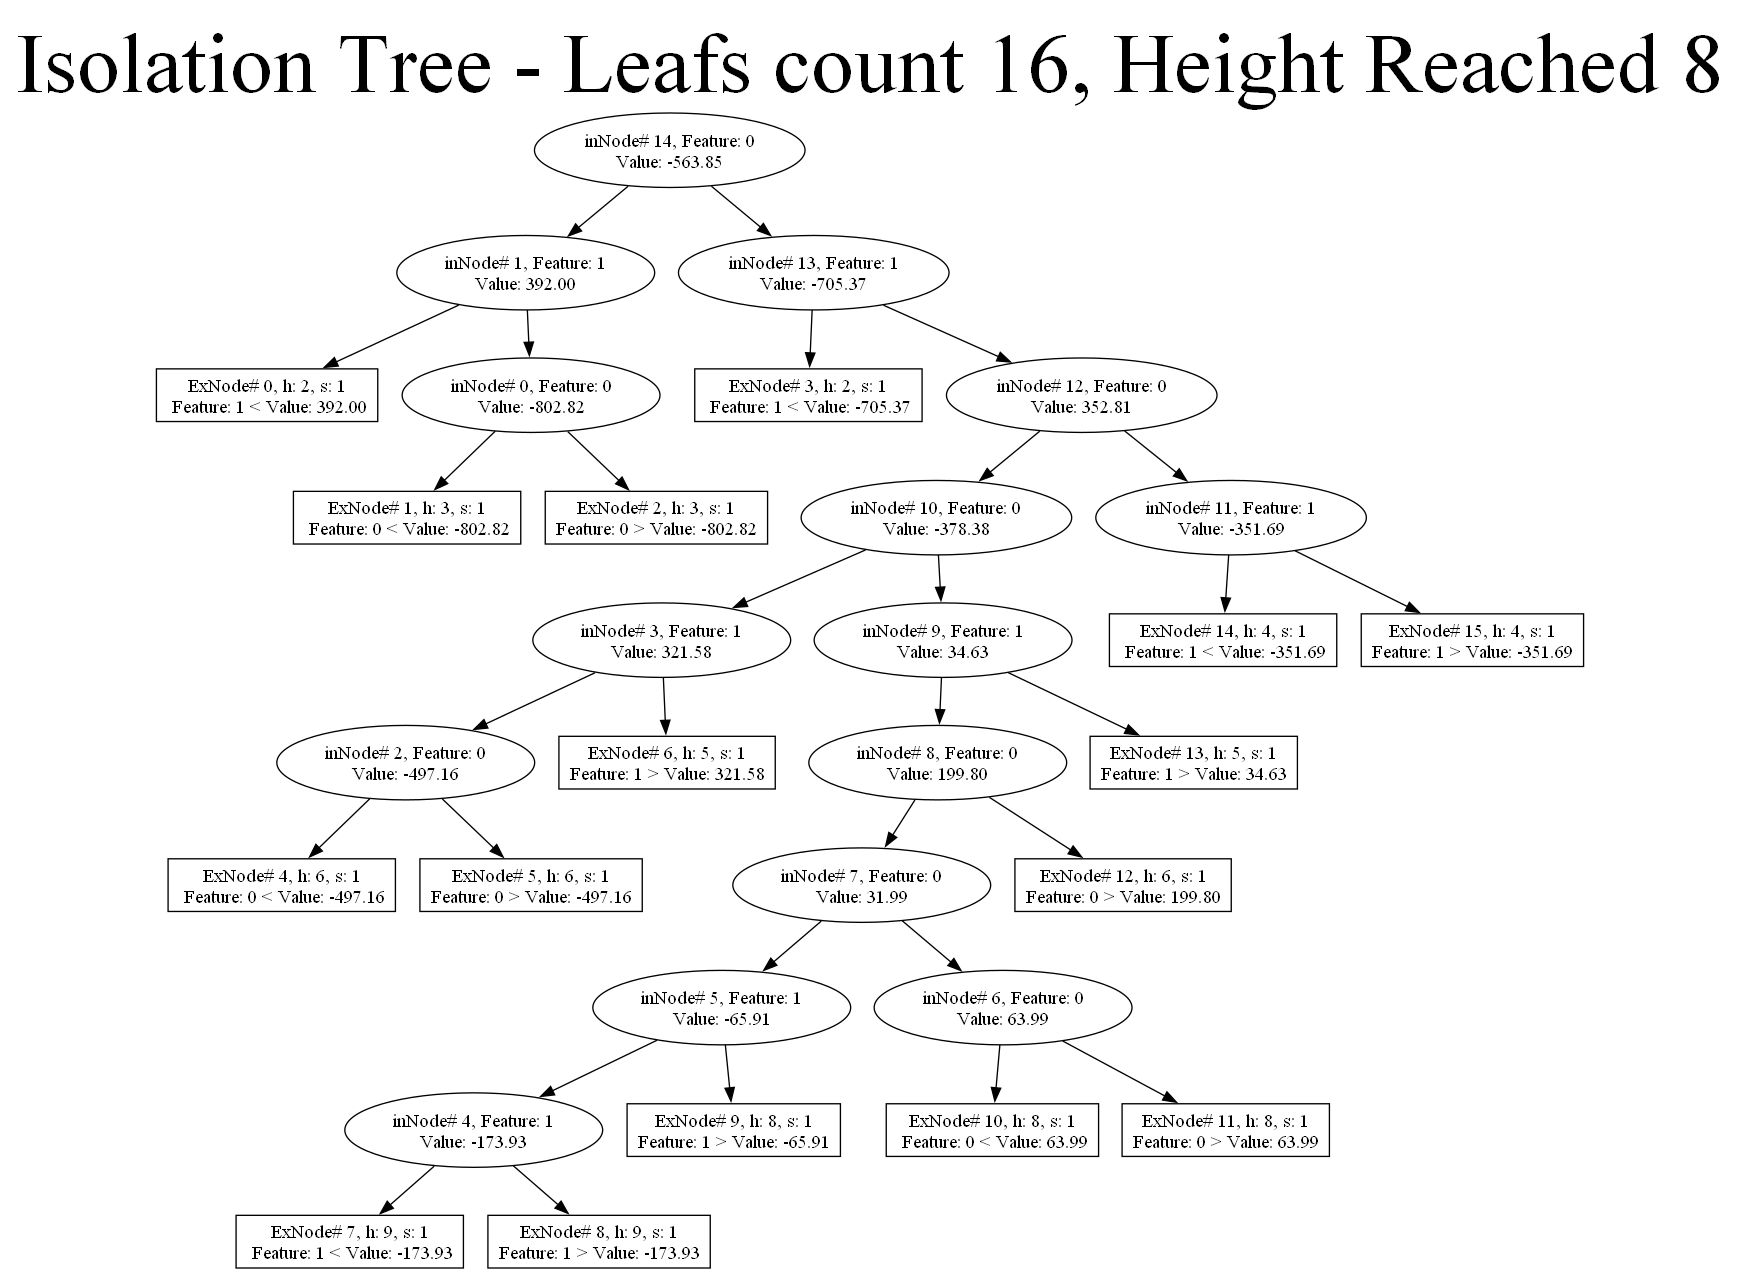
\includegraphics[width=0.5\textwidth]{resources/images/itree_pca_graph.png}
\caption{Visualization of an iTree with PCA}
\label{fig:pca_itree}
\end{figure}

\begin{figure}[htbp]
\centering
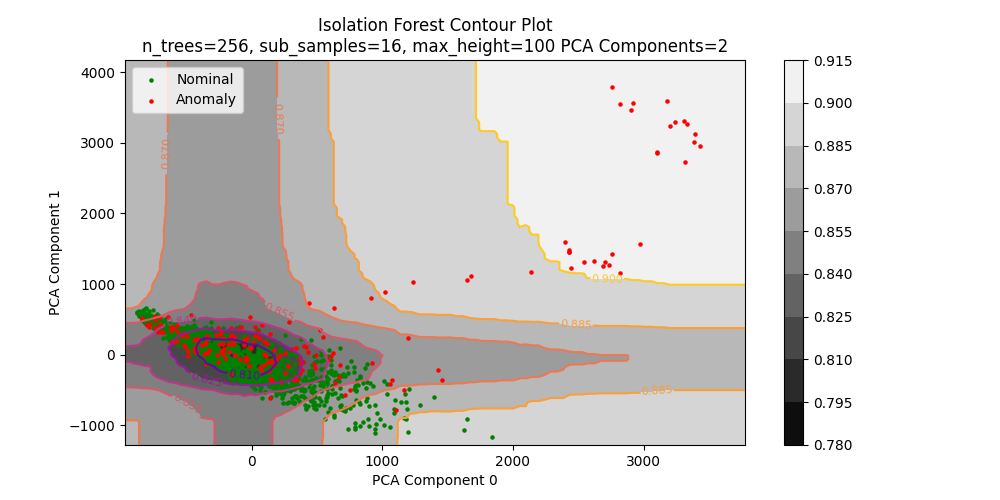
\includegraphics[width=0.5\textwidth]{resources/images/pca_contour_plot.png}
\caption{Contour plot of anomaly scores with PCA}
\label{fig:pca_contour}
\end{figure}

The dimensionality reduction techniques did not significantly improve the anomaly detection performance of the Isolation Forest algorithm on this dataset.
